%%%%%%%%%%%%%%%%%%%%%%%%%%%%%%%%%%%%%%%%%%%%%%%%%%%%%%%%%%%%%%%%%%%%
%% I, the copyright holder of this work, release this work into the
%% public domain. This applies worldwide. In some countries this may
%% not be legally possible; if so: I grant anyone the right to use
%% this work for any purpose, without any conditions, unless such
%% conditions are required by law.
%%%%%%%%%%%%%%%%%%%%%%%%%%%%%%%%%%%%%%%%%%%%%%%%%%%%%%%%%%%%%%%%%%%%

\documentclass{beamer}
\usetheme[faculty=phil]{fibeamer}
\usepackage[utf8]{inputenc}
\usepackage[
  main=english
]{babel}
%% These macros specify information about the presentation
\title{Classical Black Holes} %% that will be typeset on the
\subtitle{10. Viscous Torques  } %% title page.
\author{Edward Larra\~{n}aga}
%% These additional packages are used within the document:
\usepackage{ragged2e}  % `\justifying` text
\usepackage{booktabs}  % Tables
\usepackage{tabularx}
\usepackage{tikz}      % Diagrams
\usetikzlibrary{calc, shapes, backgrounds}
\usepackage{amsmath, amssymb}
\usepackage{url}       % `\url`s
\usepackage{listings}  % Code listings
\usepackage{siunitx}
\frenchspacing
\begin{document}
\frame{\maketitle}

\AtBeginSection[]{% Print an outline at the beginning of sections
\begin{frame}<beamer>
\frametitle{Outline for Part \thesection}
\tableofcontents[currentsection]
\end{frame}}

\section{Viscous Torques}
\begin{frame}
\Huge
Viscous Torques
\end{frame}

\begin{frame}{Accretion Disk}
	\begin{itemize}
	\item If the only interaction between fluid elements is gravity, the angular momentum is conserved.
	\pause
	\item In the description of the aaccretion disk it is needed a force responsible for the redistribution of angular momentum.
	\end{itemize}
\end{frame}

\subsection{Differential Rotation}
\begin{frame}
\Huge
Differential Rotation
\end{frame}

\begin{frame}{Differential Rotation}
	\begin{itemize}
	\item Keplerian Velocity
	\[ \Omega = \Omega (r)\]
	\pause
	\item Neighboring material at different radii moves with different velocity
	\pause
	\item The disk is not a solid body. It moves with \textit{differential rotation}.
	\pause
	\item The thermal motion of the fluid molecules and the turbulent motion of the fluid produce \textit{viscous stresses}.
	\end{itemize}
\end{frame}

\begin{frame}{Differential Rotation}
	\begin{itemize}
	\item In our simple description we will consider only momentum transport in the radial direction, produced by the process known as \textit{shear viscosity}.
	\pause
	\item It appears when there are internal distortions (usually local stresses that are proportional to the local rate of strain)
	\pause
	\item Although the following is the simplest description, it can be used to describe other mechanisms of angular momentum transport such as magnetic loops that couple fluid elements at macroscopic distances across the disk.
	\end{itemize}
\end{frame}

\begin{frame}{Modeling Viscosity}
	\begin{itemize}
	\item $\lambda$: Typical scale in the accretion disk
	\pause
	\item $\tilde{v}$: typical speed in the accretion disk
	\pause
	\item As a first model, consider a uniform gas moving only in the tangential direction woth velocity $v_\phi (r)$.
	\end{itemize}
\end{frame}


\begin{frame}{Modeling Viscosity}
	\begin{center}
      \begin{figure}
      	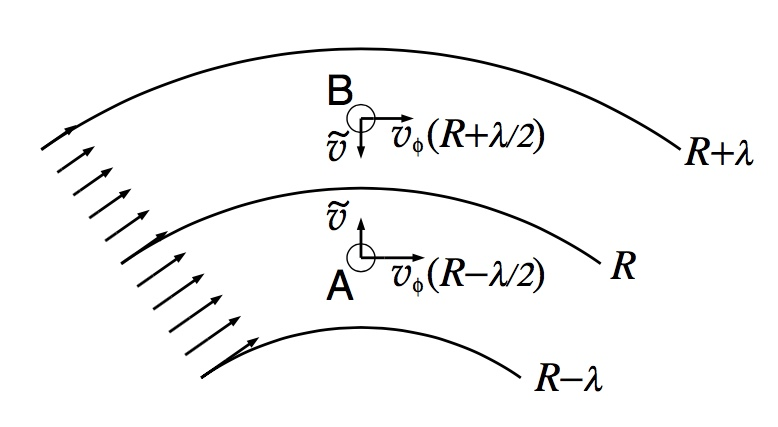
\includegraphics[scale=0.4] {figures/differentialRotation.jpeg}
      \end{figure}
	\end{center}	
\end{frame}

\begin{frame}{Modeling Viscosity}
	The only non-vanishing component of the stress tensor is the $\phi$-component of the force per unit surface of the $r=$constant surface,  
	\[\sigma_{r\phi} = -\eta \left. \frac{\partial v_\phi}{\partial r} \right|_R \]
	\pause
	$\eta$: dynamical viscosity\\
	\bigskip
	
	$v_\phi (r) = \Omega (r) r$\\
	$\frac{\partial v_\phi}{\partial r}$: velocity gradient
\end{frame}

\begin{frame}{Modeling Viscosity}
	\[\sigma_{r\phi} = -\eta R \left. \frac{\partial \Omega}{\partial r} \right|_R \]
	$\phi$-component of the force per unit surface of the $r=$constant surface.
\end{frame}

\begin{frame}{Modeling Viscosity}
	The dynamical viscosity is usually written in terms of the \textit{kinematical viscosity}, $\nu$, as $\eta = \rho \nu$\\
	\bigskip
	\pause	
	 
	The kinematical viscosity is modeled as
	\[ \nu \sim \lambda \tilde{v}\]
	\pause
	Molecular transport:\\
	$\lambda$: mean free path\\
	$\tilde{v}$: thermal speed\\
	\bigskip
	\pause
	
	Turbulent motion:\\
	$\lambda$: spatial scale (or characteristic wavelength) of the turbulence\\
	$\tilde{v}$: typical velocity of the eddies\\
\end{frame}

\begin{frame}{Modeling Viscosity}
	\[\sigma_{r\phi} = -\rho \nu R \left. \frac{\partial \Omega}{\partial r} \right|_R \]
	$\phi$-component of the force per unit surface of the $r=$constant surface.\\
	\bigskip
	\pause
	
	The net torque $(\vec{R}\times \vec{F} )$ is calculated by multiplying $\sigma_{r\phi} $ by the area of the $r=R=$constant surface, $ 2\pi R H $.\\
	\pause
	$H$: Height of the disk
\end{frame}

\begin{frame}{Modeling Viscosity}
	Net torque on the outer ring due to the inner one	.
	\pause
	\[ \textrm{Torque } = R \times 2\pi R H \times \sigma_{r\phi} \] 
	\pause
	\[\textrm{Torque } = -2 \pi R^3 H \rho \nu  \left. \frac{\partial \Omega}{\partial r} \right|_R \]
\end{frame}

\begin{frame}{Modeling Viscosity}
	Using the surface mass density, 
	\pause
	\[ \Sigma = \int_0^H \rho(r) dz = \rho H \] 
	\pause
	\[\textrm{Torque } = -2 \pi R^3 \Sigma \nu  \left. \frac{\partial \Omega}{\partial r} \right|_R \]
\end{frame}


\begin{frame}{Modeling Viscosity}
	We define the torque on the inner ring by the outer one at the coordinate $r$ as the function, 
	\pause
	\[G(r) = 2 \pi r^3 \Sigma \nu \frac{\partial \Omega}{\partial r}\]
	\begin{itemize}
	\item If $\frac{\partial \Omega}{\partial r}=0$\\ 
	\pause
	$\rightarrow$ Rigid body rotation\\
	\pause
	$\rightarrow$ No torque
	\pause
	
	\item If $\Omega (r)$ decreases outwards, $\frac{\partial \Omega}{\partial r}<0$,\\
	\pause
	$\rightarrow$ $G(r)<0$\\
	\pause
	$\rightarrow$ angular momentum goes from inner circles to outer circles.\\
	\pause
	$\rightarrow$ The gas slowly spirals in!
	\end{itemize}
\end{frame}

\begin{frame}{Differential viscous torque}
	\begin{center}
      \begin{figure}
      	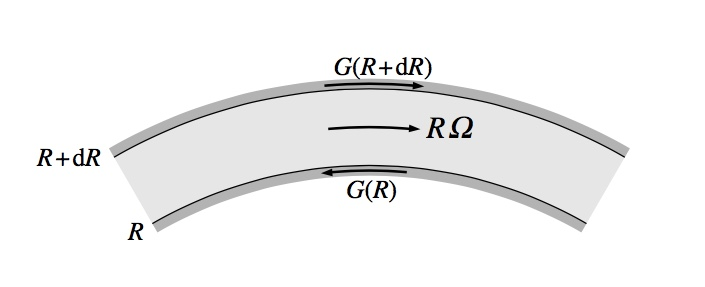
\includegraphics[scale=0.4] {figures/differentialRotation2.jpeg}
      \end{figure}
	\end{center}	
\end{frame}

\begin{frame}{Modeling Viscosity}
	The net torque on the ring between $r$ and $r+dr$ is
	\[ G(r+dr)-G(r) = \frac{\partial G}{\partial r} dr\] 
	\pause
	The work done by this torque is	
	\pause
	\[dW = \frac{\partial G}{\partial r} dr d\phi \]
	\pause
	and the associated power is
	\[P = \frac{\partial G}{\partial r} \Omega dr = \left[ \frac{\partial}{\partial r}  \left( G(r) \Omega (r) \right) - G(r) \frac{\partial \Omega}{\partial r}  \right] dr  \]
\end{frame}

\begin{frame}{Modeling Viscosity}
	\[P = \left[ \frac{\partial}{\partial r}  \left( G(r) \Omega (r) \right) - G(r) \frac{\partial \Omega}{\partial r}  \right] dr  \]
	$\frac{\partial}{\partial r}  \left( G(r) \Omega (r) \right) dr$ : Rate of \textit{convection} of the rotational energy through the gas by the torques. \\
	\pause
	Integration over the whole disk depends only on boundary conditions,
	\pause
	\[ \int_{r_{in}} ^{r_{out}} \frac{\partial}{\partial r}  \left( G(r) \Omega (r) \right) dr = \left. \Omega (r) G(r) \right|_{r_{in}} ^{r_{out}}\]
\end{frame}

\begin{frame}{Modeling Viscosity}
	\[P = \left[ \frac{\partial}{\partial r}  \left( G(r) \Omega (r) \right) - G(r) \frac{\partial \Omega}{\partial r}  \right] dr  \]
	$ - G(r) \frac{\partial \Omega}{\partial r} dr$ : Local rate of loss of mechanical energy, which is transformed into heat. \\
	\pause
	This is the viscous dissipation rate per ring of width $dr$.
	\pause
	\[ D(r) = G(r) \frac{\partial \Omega}{\partial r} dr\]
\end{frame}

\begin{frame}{Modeling Viscosity}
	Each ring of width $dr$ has two sides, with area $\sim 2\pi r dr$.\\
	\pause
	We define the dissipation rate per unit plane surface as
	\[ D(r) = \frac{ G(r) \frac{\partial \Omega}{\partial r} dr }{2 (2\pi r dr)}\]
	\pause
	\[D(r) = \frac{1}{2} \nu \Sigma \left( r \frac{\partial \Omega}{\partial r} \right)^2 \]
\end{frame}

\begin{frame}{Modeling Viscosity}
	\[D(r) = \frac{1}{2} \nu \Sigma \left( r \frac{\partial \Omega}{\partial r} \right)^2 \]
	\pause
	$D(r)\geq 0$ always $\rightarrow$ it always dissipate.\\
	\pause
	The zero corresponds to the rigid body, $\left( \frac{\partial \Omega}{\partial r}  = 0 \right)$
\end{frame}

\begin{frame}{Modeling Viscosity}
	\[D(r) = \frac{1}{2} \nu \Sigma \left( r \frac{\partial \Omega}{\partial r} \right)^2 \]
	\pause
	Using the Keplerian  angular velocity,
	\[ \Omega = \Omega_k (r) = \sqrt{\frac{GM}{r^3}} \]
	\pause
	\[D(r) = \frac{9}{8} \nu \Sigma \frac{GM}{r^3} \]
\end{frame}


\subsection{Radial Structure Evolution}    

\begin{frame}
\Huge
Radial Structure Evolution
\end{frame}

\begin{frame}{Radial Structure Evolution}
	In order to describe the radial structure of disk and its evolution we will use cylindrical coordinates $(r, \phi, z)$.\\
	\pause
	Angular velocity:
	\[ \Omega = \Omega_k (r) = \sqrt{\frac{GM}{r^3}} \]
	\pause
	Tangential velocity:
	\[v_\phi = r \Omega_k (r)\]
	\pause
	Small radial \textit{drift} velocity: $v_r = v_r (t,r) < 0 $ (negative for accretion)\\
	\pause
	Surface mass density: $\Sigma = \Sigma (t,r)$
\end{frame}

\begin{frame}{Radial Structure Evolution}
	Consider m.\\
	\pause	
	Mass: $2\pi r  dr \Sigma$\\
	\pause
	Total angular momentum: $(2\pi r dr \Sigma) r^2 \Omega$
	\pause
	\bigskip
	
	Rate of change of mass:
	\[ \frac{\partial }{\partial t} \left( 2\pi r  dr \Sigma \right) \cong -2\pi dr \frac{\partial}{\partial r} \left( r \Sigma v_r \right)\] 
	 \pause
	 In the limit $dr \rightarrow 0$ this gives the mass conservation equation
	 \[ r \frac{\partial \Sigma}{\partial t} + \frac{\partial}{\partial r} \left( r \Sigma v_r \right) = 0\] 
\end{frame}

\begin{frame}{Radial Structure Evolution}
	Rate of change of the total angular momentum:
	\[ \frac{\partial }{\partial t} \left( 2\pi r dr \Sigma r^2 \Omega \right) \cong -2\pi dr \frac{\partial}{\partial r} \left( r \Sigma v_r r^2 \Omega \right) + \frac{\partial G}{\partial r} dr \] 
	 \pause
	 In the limit $dr \rightarrow 0$ this gives the momentum conservation equation
	 \[ r \frac{\partial }{\partial t} \left( \Sigma r^2 \Omega \right) + \frac{\partial}{\partial r} \left( r \Sigma v_r  r^2 \Omega\right) = \frac{1}{2\pi} \frac{\partial G}{\partial r}\] 
\end{frame}

\begin{frame}{Radial Structure Evolution}
	Equations determining the radial structure of the accretion disk:
	\[ r \frac{\partial \Sigma}{\partial t} + \frac{\partial}{\partial r} \left( r \Sigma v_r \right) = 0\] 
	\[ r \frac{\partial }{\partial t} \left( \Sigma r^2 \Omega \right) + \frac{\partial}{\partial r} \left( r \Sigma v_r  r^2 \Omega\right) = \frac{1}{2\pi} \frac{\partial G}{\partial r}\] 
	\[G(r,t) = 2\pi r \nu \Sigma r^2  \frac{\partial \Omega}{\partial r}\]
	\[\textrm{Equation for the kinematical viscosity } \nu\]
\end{frame}

\begin{frame}{Radial Structure Evolution}
	Combining the equations determining the radial structure of the accretion disk and assuming that $\frac{\partial \Omega}{\partial t} = 0 $, we obtain
	\[ r \Sigma v_r \frac{\partial}{\partial r} \left( r^2 \Omega\right) = \frac{1}{2\pi} \frac{\partial G}{\partial r}\] 
	\pause
	Eliminating the velocity, $v_r$, we have
	\[ r \frac{\partial \Sigma}{\partial t} = -\frac{\partial }{\partial r} \left[ \frac{1}{2\pi \frac{\partial \left( r^2 \Omega\right)}{\partial r}  } \frac{\partial G}{\partial r} \right]\] 
\end{frame}

\begin{frame}{Radial Structure Evolution}
	Using the Keplerian angular velocity we obtain the equation for the time evolution of the surface mass density
	\pause
	\[ \frac{\partial \Sigma}{\partial t} = \frac{3}{r} \frac{\partial }{\partial r} \left[ r^{1/2} \frac{\partial }{\partial r} \left( \nu \Sigma r^{1/2}\right) \right]\] 
	\pause
	This is a \textit{nonlinear diffusion equation} for $\Sigma$ and one needs to know the function $\nu$ to solve it.\\
	\pause
	The radial velocity becomes 
	\[v_r = - \frac{3 }{\Sigma r^{1/2}} \frac{\partial }{\partial r} \left[ \nu \Sigma r^{1/2}\right]\]
\end{frame}

\begin{frame}{Example of Viscosity}
	Consider the particular case in which $\nu=$constant.
	\pause
	\[ \frac{\partial }{\partial t} \left( \Sigma r^{1/2} \right) = \frac{3\nu }{r} \left( r^{1/2}  \frac{\partial }{\partial r} \right)^2 \left( \Sigma r^{1/2}\right) \] 
\end{frame}

\begin{frame}{Example of Viscosity}
	Change $s = 2r^{1/2}$
	\pause
	\[ \frac{\partial }{\partial t} \left( \Sigma r^{1/2} \right) = \frac{12\nu }{s^2} \frac{\partial ^2 }{\partial s^2}  \left( \Sigma r^{1/2}\right) \] 
	\pause
	Now consider $\Sigma r^{1/2} = T(t) S(s)$,
	\pause
	\[ \frac{1}{T} \frac{dT}{dt}= \frac{12\nu}{s^"} \frac{d^2 S}{ds^2}= -\lambda^2 = \textrm{constant} \]
	\pause
	$T$: Exponential function\\
	$S$: Bessel function
\end{frame}

\begin{frame}{Example of Viscosity}
	The solution of this equation considering the initial distribution
	\[\Sigma(r,t=0) = \frac{m}{2\pi r_0} \delta (r-r_0)\]
	\pause
	is the function
	\[\Sigma(x,\tau) = \frac{m}{\pi r_0^2} \tau^{-1} x^{-1/4} \exp{\left[-\frac{1+x^2}{\tau}\right] } I_{1/4} \left( \frac{2x}{\tau} \right) \]
	\pause
	$I_{1/4} (z)$: Modified Bessel function\\
	$x=\frac{r}{r_0}$\\ 
	$\tau = \frac{12\nu t} {r_0^2}$
\end{frame}

\begin{frame}{Formation of the Accretion Disk}
	\begin{center}
      \begin{figure}
      	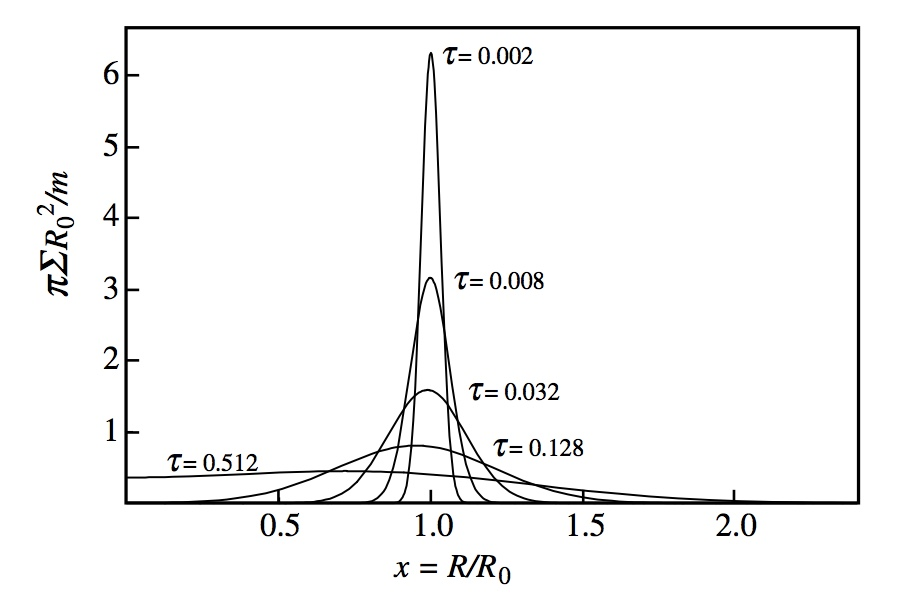
\includegraphics[scale=0.3] {figures/diskRadialStructure.jpeg}
      \end{figure}
	\end{center}	
\end{frame}


\subsection{The $\alpha$-Prescription for Viscosity}    

\begin{frame}
\Huge
The $\alpha$-Prescription for Viscosity
\end{frame}

\begin{frame}{The $\alpha$-Prescription for Viscosity}
	
\end{frame}

\section{The $alpha$-Prescription for Viscosity}    
\begin{darkframes}

\begin{frame}
\Huge
The $alpha$-Prescription for Viscosity
\end{frame}

\begin{frame}{The $alpha$-Prescription for Viscosity}
	The transferred material has a high specific angular momentum. Therefore, accretion is not a direct process.\\
	\pause
	
	As seen from the BH, the matter spreads as from a noozzle rotating around the center of mass.\\
	\pause
	\bigskip
	
	$v_\parallel $ : parallel component of the velocity with respect to the line of centers.\\
	$v_\perp $ : perpendicular component of the velocity with respect to the line of centers.
\end{frame}

\end{darkframes}

\begin{frame}{Formation of the Accretion Disk}
	\begin{center}
      \begin{figure}
      	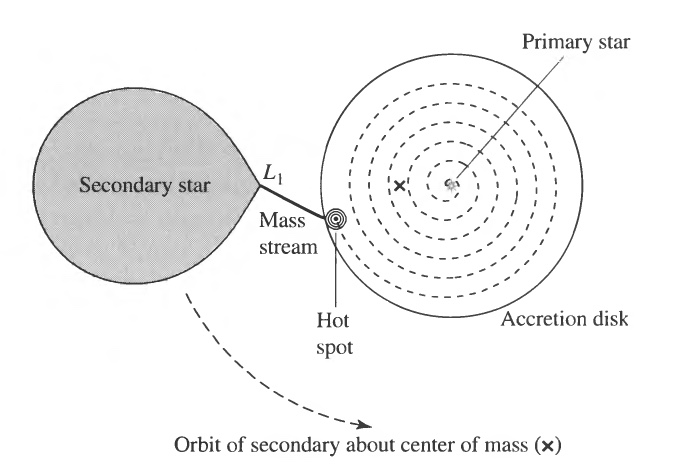
\includegraphics[scale=0.4] {figures/diskFormation.jpeg}
      \end{figure}
	\end{center}	
\end{frame}

\begin{darkframes}

\begin{frame}{Formation of the Accretion Disk}
	\[v_\parallel \lesssim c_s \]
	\pause
	$c_s$ : speed of sound in the envelope of the star.\\
	\pause
	For normal stellar envelope temperatures, $(<10^5 \textrm{ K}) $;
	\pause
	$c_s \lesssim 10 \textrm{ km/s}$
\end{frame}

\begin{frame}{Formation of the Accretion Disk}
	\[v_\perp \sim b\omega = \frac{2\pi b}{\tau} \]
	\pause
	Using
	\[ b \approx a \left[ 0.500 - 0.227 \log_10 \left( q \right) \right] \]

	\[ a = 3.5 \times 10^{10} \left( \frac{M}{M_{\odot\ }} \right)^{1/3} \left(1+q\right)^{1/3} \tau_{hr}^{2/3} \textrm{ [cm]} \]
	\pause
	we get
	\[v_\perp \gtrsim 305.6 \left( \frac{M}{M_{\odot\ }} \right)^{1/3} \left(1+q\right)^{1/3} \tau_{hr}^{-1/3} \textrm{ [km/s]}\]
\end{frame}

\begin{frame}{Formation of the Accretion Disk}
	\[v_\parallel \lesssim c_s \lesssim 10 \textrm{ km/s} \]
	\[v_\perp \gtrsim 305.6 \left( \frac{M}{M_{\odot\ }} \right)^{1/3} \left(1+q\right)^{1/3} \tau_{hr}^{-1/3} \textrm{ [km/s]}\]
	\pause
	\[v_\perp \gtrsim 104.2 \left( \frac{M}{M_{\odot\ }} \right)^{1/3} \left(1+q\right)^{1/3} \tau_{days}^{-1/3} \textrm{ [km/s]}\]
	\pause 
	\[v_\perp \gg v_\parallel \]
\end{frame}

\begin{frame}{Formation of the Accretion Disk}
	\begin{itemize}
	\item A particle (or parcel of gas) is released form rest at the point $L_1$, i.e. pressure effects are neglected.
	\pause
	\item Because of the motion of the star, this particle is moving with velocity $v_\perp $ as seen from the BH.
	\pause
	\item The particle will describe an elliptical trajectory around the BH but the presence of the star will make this ellipse to precess slowly.
	\end{itemize}
\end{frame}

\begin{frame}{Formation of the Accretion Disk}
	\begin{itemize}
	\item In the stream of accreting particles, their orbits will intersect, resulting in dissipation of energy via collisions.
	\pause
	\item However, angular momentum will be conserved in this collisions.
	\pause
	\item Hence, particles will go into the trajectories with minimum energy for a given angular momentum,
	\pause
	i.e. circular orbits!
	\pause
	\item This process is called \textit{circularization}.
	\pause
	\item The radius of the resulting circular orbit is called \textit{circularization radius}, $r_{circ}$.
	\end{itemize}
\end{frame}

\begin{frame}{Formation of the Accretion Disk}
	$\Omega_k$: Keplerian angular velocity in the circular orbit\\
	\pause
	$ v_\phi$: Tangential velocity in the circular orbit
	\pause
	\[ r_{circ} \Omega_k^2 \left( r_{circ} \right) = \frac{v_\phi^2 \left( r_{circ} \right)}{r_{circ}} = \frac{GM}{r_{circ}^2} \]
	\pause
	\[v_\phi \left( r_{circ} \right) = \sqrt{\frac{GM}{r_{circ}}}\]
\end{frame}

\begin{frame}{Formation of the Accretion Disk}
	Conservation of angular momentum
	\pause
	\[ r_{circ} v_\phi = b^2 \omega\]
	\pause
	\[ \frac{r_{circ}}{a} = \frac{4 \pi^2}{GM\tau} a^3 \left( \frac{b}{a} \right)^4 \]
	\pause
	and using Kepler's third law,
	\[\frac{r_{circ}}{a} = (1+q) \left( \frac{b}{a} \right)^4 \]
	\pause
	\[\frac{r_{circ}}{a} = (1+q)  \left[0.500 - 0.227 \log_{10} q \right]^4 \]
\end{frame}

\begin{frame}{Formation of the Accretion Disk}
	\[r_{circ} = (1+q)^{4/3}  \left[0.500 - 0.227 \log_{10} q \right]^4 \left( \frac{M}{M_{\odot\ }} \right)^{1/3} \tau_{days}^{2/3} \textrm{ } \left[ R_{\odot\ } \right] \]
\end{frame}

\begin{frame}{Formation of the Accretion Disk}
	\begin{itemize}
	\item The stream of gas moves in a ring with $r=r_{circ}$.
	\pause
	\item In the ring the particles have collisions, shocks, viscous dissipation and other processes that transform some of the potential energy into heat (producing radiation).
	\pause
	\item However, this release of energy needs the loosing of angular momentum.
	\pause
	\item In the absence of external torques, the only possible process is a \textit{transfer of angular momentum} from inner regions outwards by internal torques.
	\pause
	\item The redistribution of angular momentum makes particles in the outer parts move outwards (gaining angular momentum) and the particles in the inner particles spiral inwards.
	\end{itemize}
\end{frame}

\begin{frame}{Formation of the Accretion Disk}
	\begin{itemize}
	\item The accretion disk will extend from $r_{in} \geq r_{ISCO}$ up to $r_{out} \leq b$
	\pause
	\item Viscous torques may be modeled using different processes:
	\begin{itemize}
	\pause
	\item Viscous torques due to differential rotation in the accretion disk (produced by the thermal motion of the fluid molecules). This is a local mechanism for angular momentum transport
	\pause
	\item Magnetic loops that couple fluid elements located at macroscopic distances across the disk. This is a non-local mechanism for angular momentum transport.
	\pause
	\item Turbulence in the fluid may be an origin of angular momentum transport. Turbulence may be produced by mechanisms as Themally driven convection, Pure hydrodynamic instabilities or Magnetohydrodynamic (MHD) turbulence.
	\end{itemize}
	
	\pause
	\item However, this release of energy needs the loosing of angular momentum.
	\pause
	\item In the absence of external torques, the only possible process is a \textit{transfer of angular momentum} from inner regions outwards by internal torques.
	\pause
	\item The redistribution of angular momentum makes particles in the outer parts move outwards (gaining angular momentum) and the particles in the inner particles spiral inwards.
	\end{itemize}
\end{frame}






\end{darkframes}
\begin{frame}{Temperature of the gas in the accretion structure}
	\begin{center}
      \begin{figure}
      	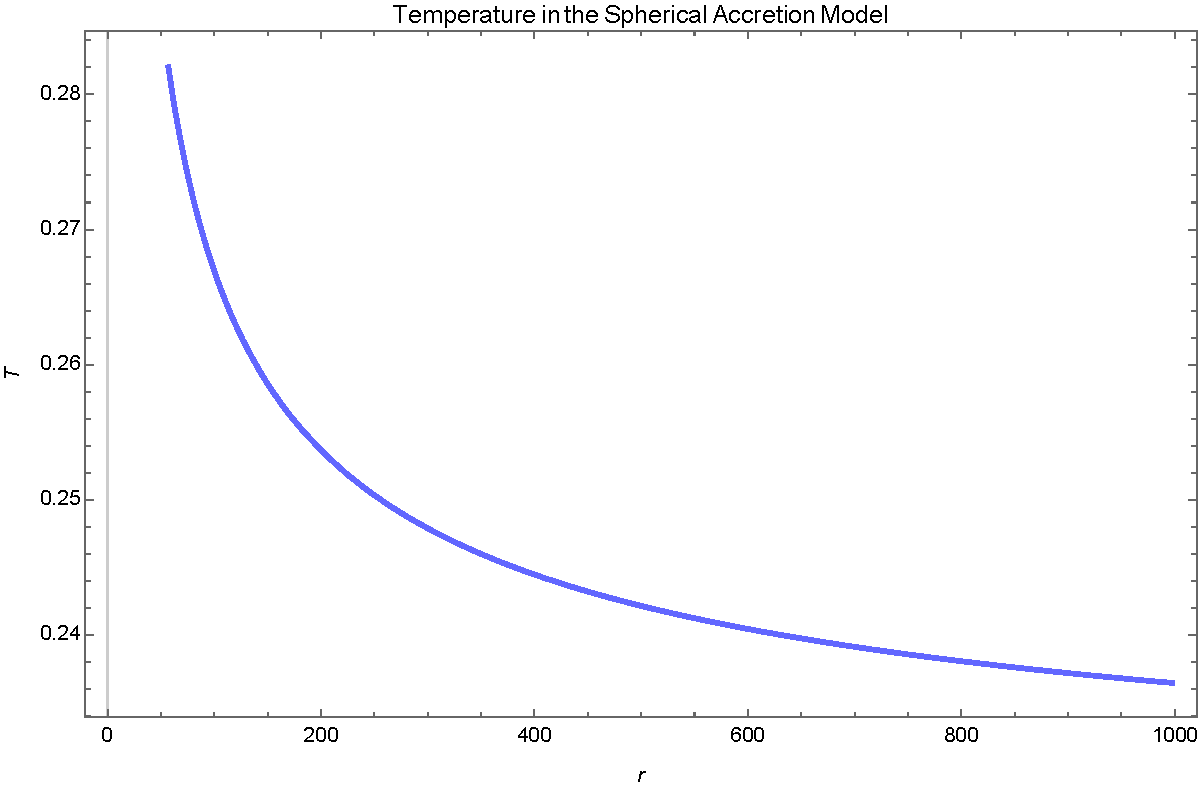
\includegraphics[scale=0.45] {figures/Temperature.pdf}
      \end{figure}
	\end{center}	
\end{frame}

\begin{darkframes}

\begin{frame}{Next Lecture}
  	\Large
	{10. Accretion Disks. Detailed Description}
\end{frame}

  
\end{darkframes}
\end{document}
